\hypersetup{pageanchor=false} 

\begin{titlepage}
\phantom.

\bigskip

\begin{center}
{\sc\LARGE Žilinská Univerzita v Žiline}
\medskip

{\sc\Large Fakulta riadenia a informatiky}

\vfill\vfill\vfill\vfill

{\sc\LARGE Bakalárska práca}

\medskip

{\large Študijný odbor: {\bf Informatika}}
\end{center}


\vfill\vfill\vfill\vfill


\phantom.\hfill

\begin{center}
{\large\bf Oľga Chovancová}

\medskip

{\large\bf Vizualizácia dát získaných pomocou SCADA systémov s využitím HTML 5 štandartov}

\medskip

Vedúci: {\bf Ing. Juraj Veverka}\\
Tútor	\textbf{Ing. Patrik Hrkút, PhD.}
\medskip
 
\hfill
Reg.č. 5/2014
\hfill
Máj 2015
\hfill\phantom.
\end{center}

\hspace{1.7cm}\phantom.

\vspace{2.9cm}

\phantom.
\end{titlepage}
%%%%%%%%%%%%%%%%%%%%%%%%%%%%%%%%%%%%%%%%%%%%%%%%%%%%%%%%%%%%%%%%%%%%%%%%%%%%%%%%%%%%%%%%%%%%%%%%%%%%%%%%%%%%%%%%%%%%%%%%%%%%%%%%%%%%%%%%%%%%%%%%%%%%%%%%%%%%%%%%%%%%%%%%%%%%%%%%%%%%%%%%%%%%%%%%%%%%%%%%%%%%%%%%%%%%%%%%%%%%%%%%%%%%%%%%%%%%%%%%%%%%%%%%%%%%%%%%%%

%%%%%%%%%%%%%%%%%%%%%%%%%%%%%%%%%%%%%%%%%%%%%%%%%%%%%%%%%%%%%%%%%%%%%%%
\newpage

\centerline{\bf Prehlásenie}

\vspace{2em}

\noindent
Prehlasujem, že som túto prácu napísala samostatne a že som uviedola
všetky použité pramene a literatúru, z~ktorých som čerpala. 

\vspace{2em}

\noindent
V~Žiline, dňa 15.05.2015
\hfill
Oľga Chovancová

\newpage

\centerline{\bf Poďakovanie}

\vspace{2em}

\noindent
%Prehlasujem, že som túto prácu napísala samostatne a že som uviedola
%všetky použité pramene a literatúru, z~ktorých som čerpala. 

\vspace{2em}

\noindent
V~Žiline, dňa 15.05.2015
\hfill
Oľga Chovancová



%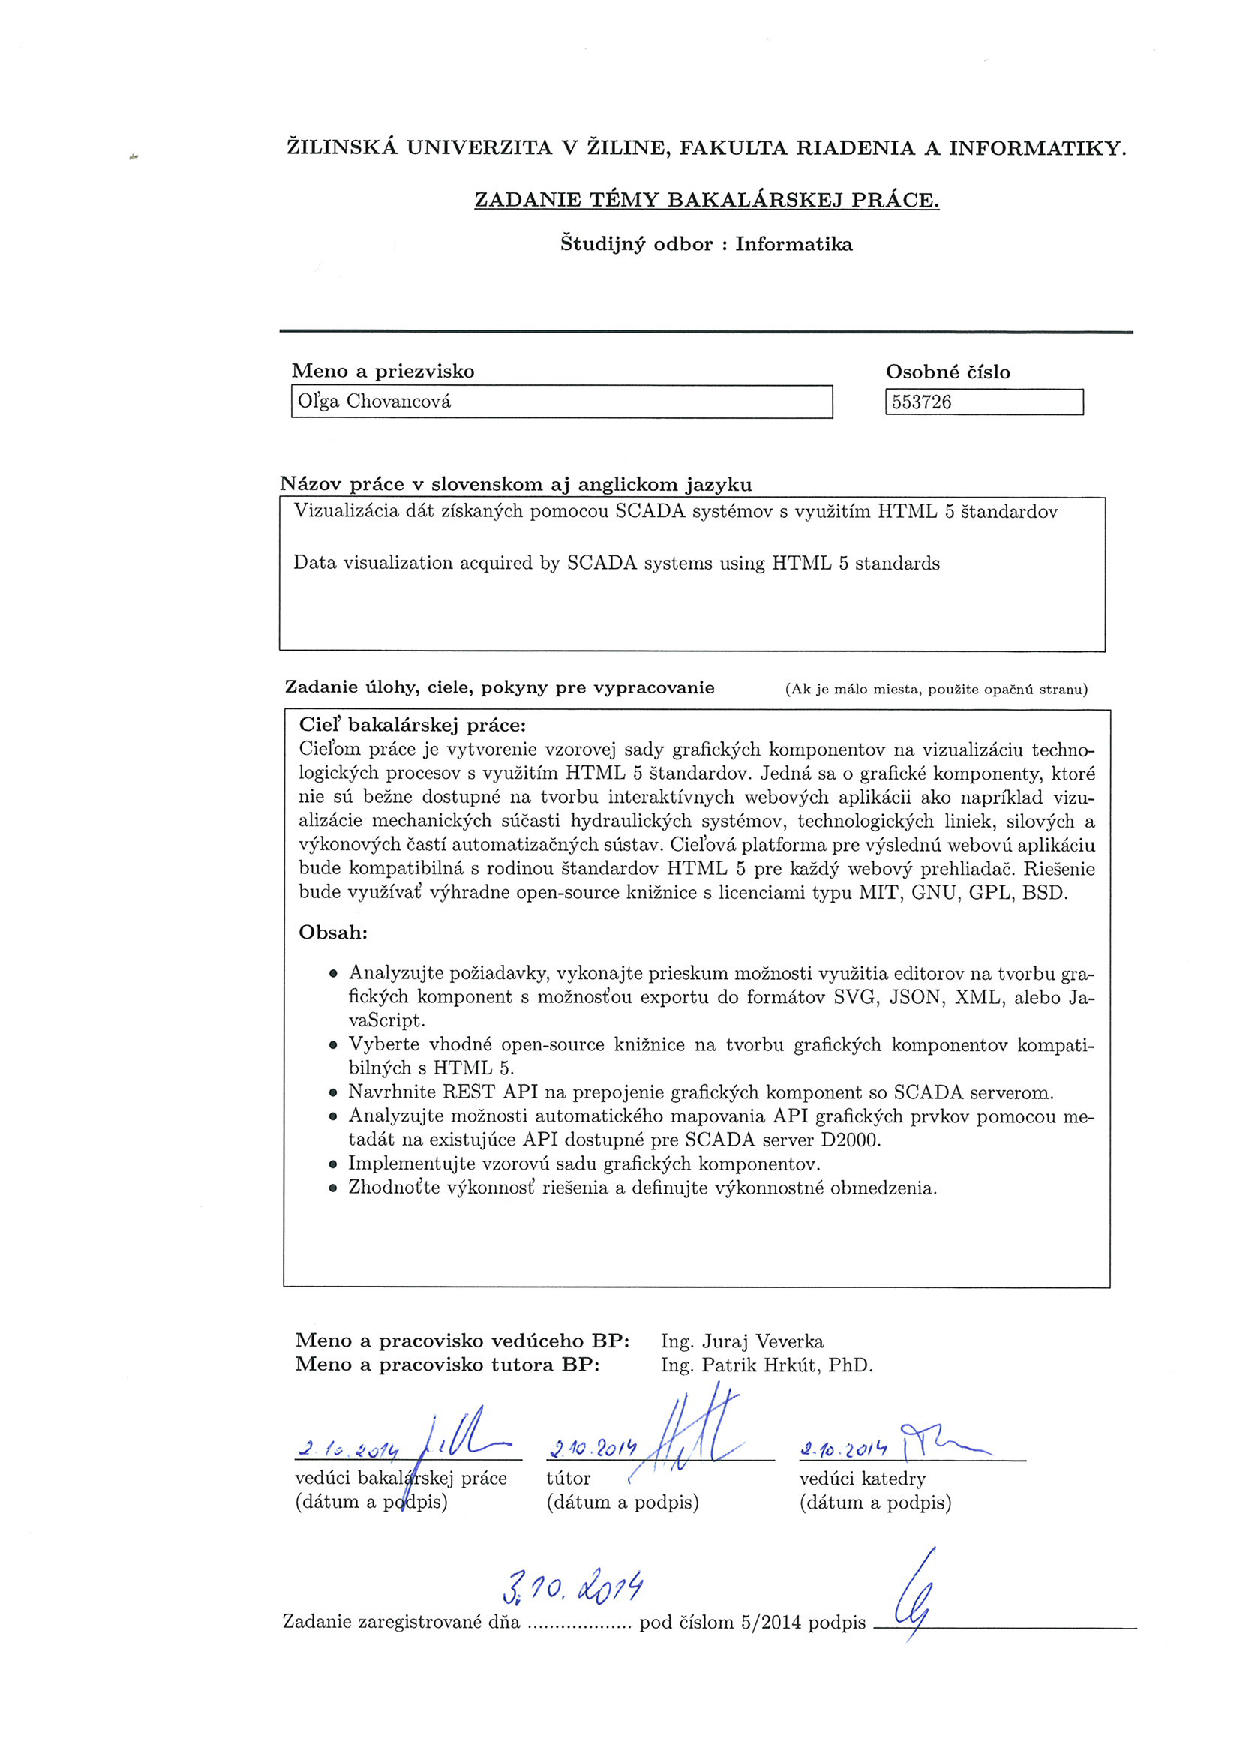
\includepdf[pages={1}]{zadanie_temy_bakalarskej_prace.pdf}

	

%--------------------------------------------------------------------------------------
%%% slovensky abstrakt

\begin{abstract}

\noindent
{\sc Chovancová Oľga:} {\em Vizualizácia dát získaných pomocou SCADA systémov s využitím HTML 5 štandartov}
[Bakalárska práca] 

\noindent
Žilinská Univerzita v~Žiline,  
Fakulta riadenia a informatiky,  
Katedra softvérových technológií.

\noindent  
Vedúci: Ing. Juraj Veverka 
 
\noindent
Tútor	Ing. Patrik Hrkút, PhD.

\noindent  
Stupeň odbornej kvalifikácie:
študentka na Fakulte riadenia a informatiky, odbor Informatika
%Inžinier v študijnom odbore Telekomunikačné siete, na Elektrotechnickej fakulte na Žilinskej univerzite v Žiline. 


\bigskip

Obsahom práce je vzorová sada grafických komponentov na vizualizáciu technologických procesov s využitím HTML 5 štandardov. Jedná sa o grafické komponenty, ktoré nie sú bežne dostupné na tvorbu interaktívnych webových aplikácii ako napríklad vizualizácie mechanických súčasti hydraulických systémov, technologických liniek, silových a výkonových častí automatizačných sústav. Návrh interface, pomocou, ktorého budú tieto komponenty komunikovať so serverovou časťou SCADA systému. Cieľová platforma pre výslednú webovú aplikáciu bude kompatibilná s rodinou štandardov HTML 5 pre každý webový prehľadávač. 
\end{abstract}


%--------------------------------------------------------------------------------------
%%% anglicky abstrakt


\selectlanguage{english}
\begin{abstract}

\noindent
{\sc Chovancová Oľga:} {\em Data visualization acquired by SCADA systems using HTML5 standarts}
[Bacalar thesis] 

\noindent
University of Žilina,  
Faculty of Management Science and Informatics, 
Department of TODO.
 
\noindent
Tutor:  Ing. Juraj Veverka.
Tutor:  Ing. Patrik Hrkut, PhD.
 
\noindent
Qualification level:

%
%Engineer in field University of Zilina, Faculty of Telecommunication, Fixed networks.
%Solution Design Architect %- member of team who develops system D2000. 

\noindent
 TODO

\bigskip

The main idea of this ... TODO

\end{abstract}
\selectlanguage{slovak}
